\documentclass[11pt,a4paper]{article}
\usepackage[margin={2.6cm,2.6cm}]{geometry}
\usepackage{lmodern}
\usepackage{microtype}
\usepackage{enumitem}
\usepackage{array}
\usepackage[spanish,es-tabla]{babel}
\usepackage[utf8]{inputenc}
\usepackage[T1]{fontenc}
\usepackage{amsmath, amsthm, amsfonts}
\usepackage{hyperref}
\usepackage{xcolor}
\usepackage{graphicx}
 \usepackage{float}
\usepackage{listings}
\usepackage{fontawesome5}
\usepackage{dirtree}

\spanishdecimal{.}
\definecolor{azuluc}{HTML}{1F4E79}
\definecolor{grisclaro}{HTML}{F4F6F8}
\definecolor{gris}{HTML}{586069}
\definecolor{verde}{HTML}{2E7D32}
\definecolor{rojo}{HTML}{A94442}
\definecolor{git}{HTML}{F1502F}
\definecolor{morado_ubuntu}{RGB}{48, 10, 36}       % Fondo morado oscuro de Ubuntu GNOME
\definecolor{verde_ubuntu}{RGB}{78, 154, 6}        % Verde para comentarios
\definecolor{cyan_ubuntu}{RGB}{52, 226, 226}       % Cian para comandos
\definecolor{amarillo_ubuntu}{RGB}{250, 240, 190}  % Amarillo para cadenas
\definecolor{rojo_ubuntu}{RGB}{220, 50, 47}        % Rojo para errores
\definecolor{verde_claro_ubuntu}{RGB}{138, 226, 52} % Verde claro para el prompt
\definecolor{azul_ubuntu}{RGB}{114, 159, 207}      % Azul para símbolos y rutas
\definecolor{gris_ubuntu}{RGB}{128, 128, 128}      % Gris para el borde del frame
\definecolor{fondo_mac}{RGB}{255, 255, 250}       % Fondo beige claro típico de macOS
\definecolor{negro}{RGB}{0, 0, 0}                 % Texto en negro
\definecolor{verde_mac}{RGB}{63, 127, 95}         % Verde para comentarios
\definecolor{azul_mac}{RGB}{0, 0, 255}            % Azul para comandos y prompt
\definecolor{rojo_mac}{RGB}{196, 26, 22}          % Rojo para errores y cadenas
\definecolor{morado_mac}{RGB}{147, 39, 143}       % Morado para emphasis (opcional)
\definecolor{gris_mac}{RGB}{200, 200, 200}        % Gris para el borde del frame
\definecolor{DarkGreen}{RGB}{0,102,0}
\definecolor{DarkYellow}{RGB}{243,220,12}

\lstdefinestyle{rstyle}{
  language=R,
  basicstyle=\ttfamily\small,
  keywordstyle=\color{azuluc}\bfseries,
  commentstyle=\color{gris},
  stringstyle=\color{verde!70!black},
  showstringspaces=false,
  frame=single,
  rulecolor=\color{gris!30},
  backgroundcolor=\color{grisclaro},
  breaklines=true,
  showspaces=false,
  tabsize=2,
    literate=
    {á}{{\'a}}1
    {é}{{\'e}}1
    {í}{{\'i}}1
    {ó}{{\'o}}1
    {ú}{{\'u}}1
    {Á}{{\'A}}1
    {É}{{\'E}}1
    {Í}{{\'I}}1
    {Ó}{{\'O}}1
    {Ú}{{\'U}}1
    {ñ}{{\~n}}1
    {Ñ}{{\~N}}1
    {ü}{{\"u}}1
    {Ü}{{\"U}}1
    {¡}{{\textexclamdown}}1
	{`}{\textasciigrave}1 
    {´}{\textquotesingle}1,
}

\lstdefinestyle{rconsole}{
  language=R,
  basicstyle=\color{rojo}\ttfamily\small,
  showstringspaces=false,
  frame=single,
  rulecolor=\color{gris!30},
  breaklines=true,
  tabsize=2,
  literate=
    {á}{{\'a}}1
    {é}{{\'e}}1
    {í}{{\'i}}1
    {ó}{{\'o}}1
    {ú}{{\'u}}1
    {Á}{{\'A}}1
    {É}{{\'E}}1
    {Í}{{\'I}}1
    {Ó}{{\'O}}1
    {Ú}{{\'U}}1
    {ñ}{{\~n}}1
    {Ñ}{{\~N}}1
    {ü}{{\"u}}1
    {Ü}{{\"U}}1
    {¡}{{\textexclamdown}}1
	{`}{\textasciigrave}1 
    {´}{\textquotesingle}1,
}

\lstdefinestyle{routput}{
  language=R,
  basicstyle=\color{azuluc}\ttfamily\small,
  showstringspaces=false,
  frame=single,
  rulecolor=\color{gris!30},
  breaklines=true,
  tabsize=2,
  literate=
    {á}{{\'a}}1
    {é}{{\'e}}1
    {í}{{\'i}}1
    {ó}{{\'o}}1
    {ú}{{\'u}}1
    {Á}{{\'A}}1
    {É}{{\'E}}1
    {Í}{{\'I}}1
    {Ó}{{\'O}}1
    {Ú}{{\'U}}1
    {ñ}{{\~n}}1
    {Ñ}{{\~N}}1
    {ü}{{\"u}}1
    {Ü}{{\"U}}1
    {¡}{{\textexclamdown}}1
	{`}{\textasciigrave}1 
    {´}{\textquotesingle}1,
}

\lstdefinestyle{mdstyle}{
  basicstyle=\ttfamily\footnotesize,
  keywordstyle=\color{azuluc}\bfseries,
  commentstyle=\color{gris},
  showstringspaces=false,
  showspaces=false,
  tabsize=2,
  frame=single,
  rulecolor=\color{gris!30},
  backgroundcolor=\color{grisclaro},
  breaklines=true,
  breakatwhitespace=false,
  % Títulos Markdown
  morecomment=[l][\color{azuluc}\bfseries]{\#},
  % Lenguajes utilizados en bloques de código
  classoffset=1,
    morekeywords={python,bash,R,latex,json,yaml},
  classoffset=0,
  % Protocolos y enlaces
  emph={http,https,ftp},
  escapeinside={-@}{@-},
  emphstyle=\color{azuluc}\underbar,   
   literate=
    {á}{{\'a}}1
    {é}{{\'e}}1
    {í}{{\'i}}1
    {ó}{{\'o}}1
    {ú}{{\'u}}1
    {Á}{{\'A}}1
    {É}{{\'E}}1
    {Í}{{\'I}}1
    {Ó}{{\'O}}1
    {Ú}{{\'U}}1
    {ñ}{{\~n}}1
    {Ñ}{{\~N}}1
    {ü}{{\"u}}1
    {Ü}{{\"U}}1
    {¡}{{\textexclamdown}}1
	{`}{\textasciigrave}1 
    {´}{\textquotesingle}1,
}

\lstdefinestyle{ubuntugnome}{
  basicstyle=\ttfamily\small\color{white},
  backgroundcolor=\color{morado_ubuntu},
  commentstyle=\color{verde_ubuntu},
  keywordstyle=\color{cyan_ubuntu},
  stringstyle=\color{amarillo_ubuntu},
  emphstyle=\color{rojo_ubuntu},
  showstringspaces=false,
  frame=single,
  rulecolor=\color{gris_ubuntu},
  breaklines=true,
  postbreak=\mbox{\textcolor{white}{$\hookrightarrow$}\space},
  % Configuración para simular el prompt de Ubuntu
  upquote=true,
  % Resaltar el prompt de usuario
  emph={user@ubuntu:~\$},
  emphstyle={\color{verde_claro_ubuntu}\bfseries},
  % Resaltar errores (ej: "command not found")
  classoffset=1,
  emph={command not found,No such file or directory,Permission denied},
  emphstyle={\color{rojo_ubuntu}},
  classoffset=0,
}

\lstdefinestyle{macterminal}{
  basicstyle=\ttfamily\small\color{negro},
  backgroundcolor=\color{fondo_mac},
  commentstyle=\color{verde_mac},
  keywordstyle=\color{azul_mac},
  stringstyle=\color{rojo_mac},
  emphstyle=\color{morado_mac},
  showstringspaces=false,
  frame=single,
  rulecolor=\color{gris_mac},
  breaklines=true,
  postbreak=\mbox{\textcolor{negro}{$\hookrightarrow$}\space},
  % Configuración para simular el prompt de macOS
  upquote=true,
  % Resaltar el prompt de usuario
  emphstyle={\color{azul_mac}\bfseries},
  % Resaltar errores (ej: "command not found")
  classoffset=1,
  emph={command not found,No such file or directory,Permission denied},
  emphstyle={\color{rojo_mac}},
  classoffset=0
}

\lstdefinestyle{windowscmd}{
  basicstyle=\ttfamily\small\color{white},
  backgroundcolor=\color{black},
  showstringspaces=false,
  frame=single,
  rulecolor=\color{gris_mac},
  breaklines=true,
  postbreak=\mbox{\textcolor{negro}{$\hookrightarrow$}\space},
  % Configuración para simular el prompt de macOS
  upquote=true,
  % Resaltar el prompt de usuario
  emphstyle={\color{azul_mac}\bfseries},
  % Resaltar errores (ej: "command not found")
  classoffset=1,
  emph={command not found,No such file or directory,Permission denied},
  emphstyle={\color{rojo_mac}},
  classoffset=0
}

\newcommand*{\vsp}{\texttt{\textvisiblespace}} % visible space
\newcommand*{\strC}{\begingroup
  \obeyspaces
  \begingroup\lccode`~=`\ %
  \lowercase{\endgroup\let~}\vsp
  \dostrC}

\newcommand{\dostrC}[1]{\textnormal{{\slshape\ttfamily#1}}\endgroup} % string constant
\newcommand{\R}{\textcolor{azuluc}{\faIcon{r-project}}}
\newcommand{\Git}{\textcolor{git}{\faIcon{git-alt}}~\!Git}
\newcommand{\GitHub}{\faIcon{github}~\!GitHub}
\newcommand{\Markdown}{Markdown~\faIcon{markdown}}
\newcommand{\checkicon}{\textcolor{verde}{\faIcon{check}}}
\newcommand{\crossicon}{\textcolor{rojo}{\faIcon{times}}}

\newtheoremstyle{exercise}{0.8em}{0.8em}{\normalfont}{}{\bfseries\color{azuluc}}{.}{0.5em}{}
\theoremstyle{exercise}
\newtheorem{exercise}{Ejercicio}




\title{\LARGE\textbf{Práctica 9: Introducción a RMarkdown}\\[0.5em]
\Large Laboratorio de Matemáticas\\
\small\ \\
\Large Grado en Ingeniería Matemática - Doble Grado en Física e Ingeniería Matemática}
\author{Miguel Beltrá Vidal}
\date{Curso 2026/27}



\begin{document}

\maketitle


\section{Objetivos}

El objetivo de esta práctica es aprender los fundamentos de R Markdown. Al finalizar, el estudiante deberá ser capaz de crear ficheros de R Markdown y exportarlos a diversos formatos como PDF y HTML.



\section{Introducción a R Markdown}

R Markdown es una herramienta gratuita y de código abierto (\emph{open source}) que permite crear documentos dinámicos combinando texto, código de programación y resultados de su ejecución.

Es especialmente útil para elaborar informes de análisis de datos, memorias de prácticas, trabajos científicos y documentación técnica. Una de sus principales ventajas es que permite integrar en un mismo documento:

\begin{itemize}
	\item Texto explicativo y fórmulas matemáticas.
	\item Código de programación.
	\item Resultados numéricos.
	\item Tablas y gráficos.
	\item Referencias bibliográficas.
\end{itemize}

Además, los resultados se pueden exportar a distintos formatos, como HTML, PDF o Word.



\subsection{Instalación de R Markdown}

Podemos instalar la librería de R Markdown con

\begin{lstlisting}[style=rconsole]
> install.packages("R Markdown")
\end{lstlisting}

Para generar documentos PDF también necesitamos disponer de una distribución de LaTeX, como por ejemplo MiKTex. Otra alternativa sencilla consiste en instalar TinyTeX:

\begin{lstlisting}[style=rconsole]
install.packages("tinytex")
tinytex::install_tinytex()
\end{lstlisting}

No es necesario instalar LaTeX para generar documentos HTML.



\subsection{Ficheros de R Markdown}

Los ficheros de R Markdown utilizan habitualmente la extensión \texttt{.Rmd}, combinación de la extensión de \R\, que es \texttt{.R}, con la extensión de \Markdown, que es \texttt{.md}.


\subsection{Elementos que componen un fichero de R Markdown}

Todo documento de R Markdown tiene tres tipos de elementos importantes:
\begin{enumerate}
	\item Un encabezado YAML (opcional) rodeado de \verb|---|.
	\item Bloques de texto con formato Markdown.
	\item Bloques de código de \R\ rodeados de \texttt{\textasciigrave\textasciigrave\textasciigrave}.
\end{enumerate}


\noindent El siguiente es el ejemplo que proporciona RStudio. Obsérvalo con atención.

\begin{center}
	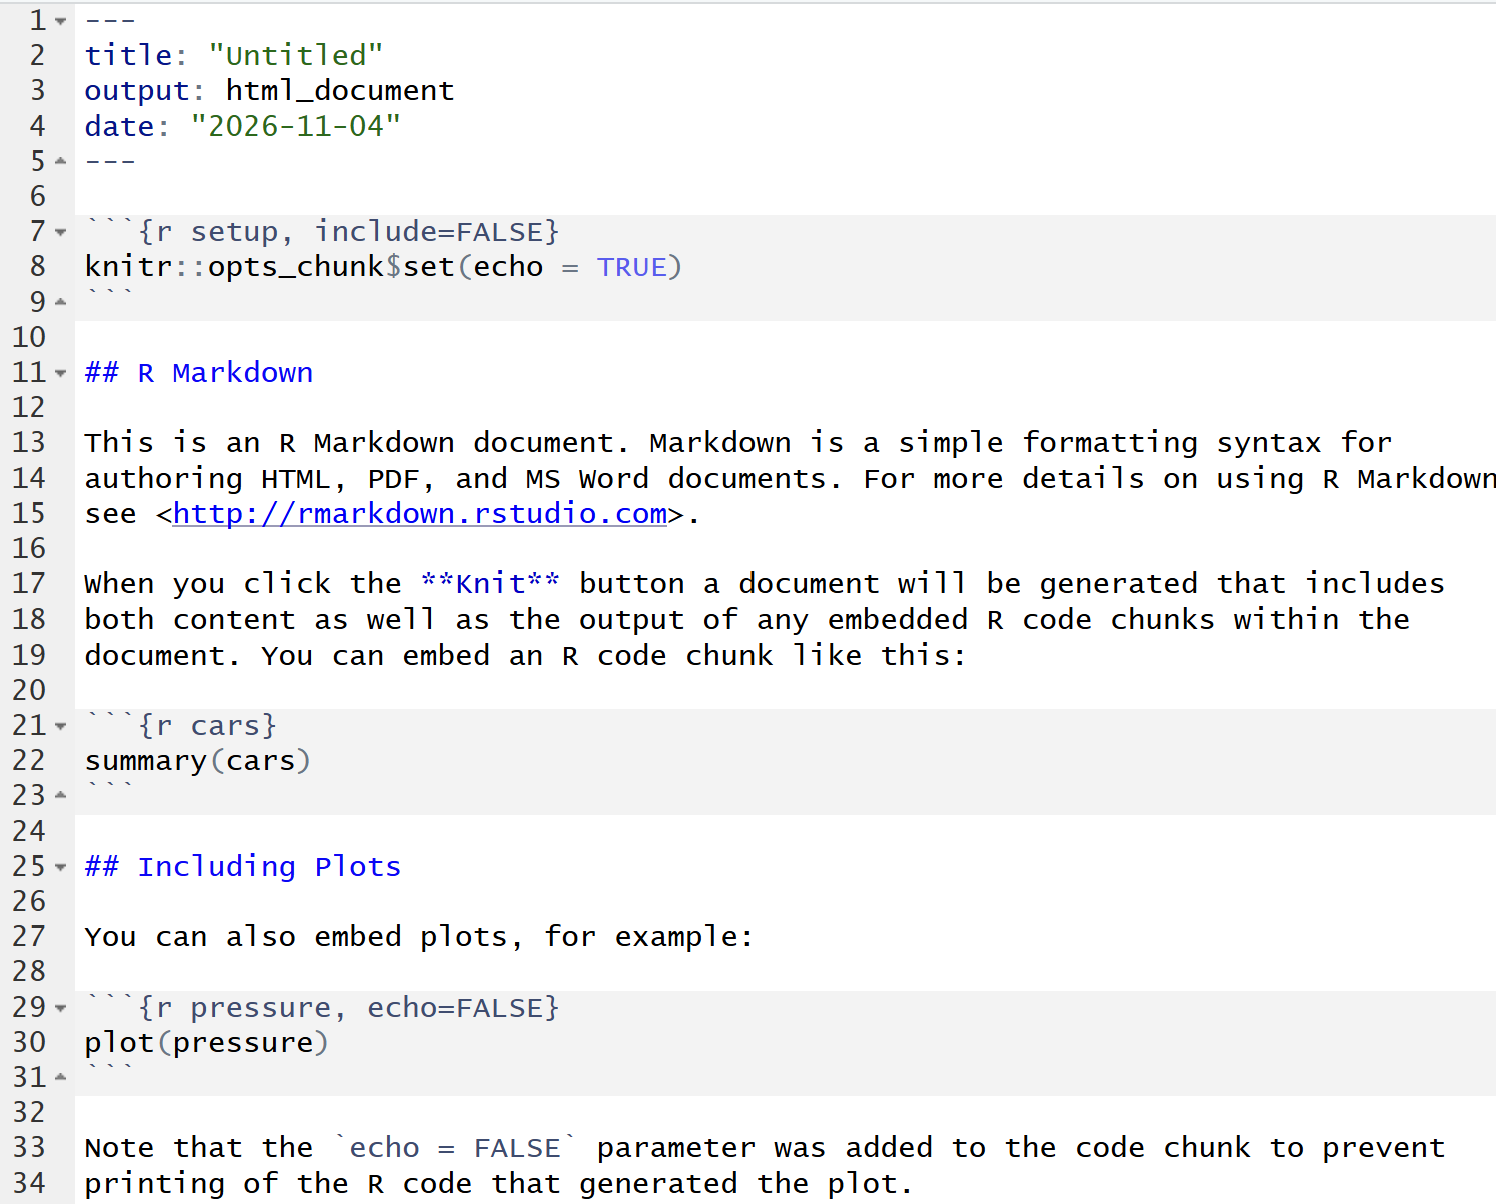
\includegraphics[width=0.85\textwidth]{images/rmarkdown_example.png}
\end{center}

\noindent A continuación se explica cada uno de los bloques.


\subsubsection{Encabezado YAML}

El nombre YAML es un acrónimo recursivo que significa \emph{YAML Ain't Markup Language}. Aparece al principio del documento, delimitado por dos líneas que contienen tres guiones (\verb|---|).

\begin{lstlisting}[style=mdstyle]
---
title: "Mi primer documento R Markdown"
author: "Nombre y apellidos"
date: "2026-11-05"
output: html_document
---
\end{lstlisting}

Los principales elementos son:
\begin{itemize}
	\item \verb|title|: título del documento.
	\item \verb|author|: autor.
	\item \verb|date|: fecha.
	\item \verb|output|: formato de salida.
\end{itemize}
Entre los formatos de salida encontramos \texttt{html\_document} o \texttt{pdf\_document}. También podemos especificar varios formatos de salida:

\begin{lstlisting}[style=mdstyle]
---
title: "Mi primer documento R Markdown"
author: "Nombre y apellidos"
output:
  html_document:
    toc: true
  pdf_document:
    toc: true
---
\end{lstlisting}



\subsubsection{Bloques de texto}

Los bloques de texto se escribirán en formato \Markdown. Revisa la práctica 4 para recordar los fundamentos de \Markdown. En próximas prácticas veremos más elementos de \Markdown\ para poder diseñar mejores documentos.


\subsubsection{Bloques de código (code chunks)}

Los bloques de código permiten incorporar instrucciones que serán ejecutadas durante la generación del documento. En R Markdown, un bloque de código \R\ tiene la siguiente estructura:

\begin{lstlisting}[style=mdstyle]
```{r}
# Código R
```
\end{lstlisting}

\noindent Por ejemplo:

\begin{lstlisting}[style=mdstyle]
```{r}
x <- seq(0, 2*pi, by=0.01)
y <- sin(x)

plot(x, y, type = "l",
     main = "Función seno",
     xlab = "x",
     ylab = "sin(x)")
```
\end{lstlisting}

Podemos insertarlos manualmente, o mediante el botón de RStudio para este propósito:

\begin{center}
	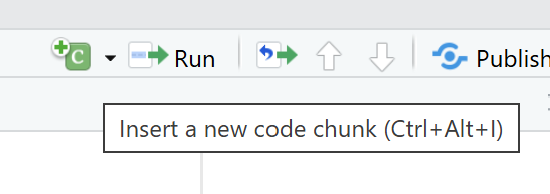
\includegraphics[width=0.3\linewidth]{images/boton_code_chunk.png}
\end{center}


\medskip

Podemos controlar cómo se muestran el código y sus resultados mediante diferentes opciones. Algunas de las más importantes son:

\begin{center}
	\begin{tabular}{|l|l|}\hline
		Opción & Descripción \\ \hline
		\verb|echo=TRUE| & Muestra el código \R. \\
		\verb|echo=FALSE| & Oculta el código \R. \\
		\verb|eval=TRUE| & Ejecuta el código. \\
		\verb|eval=FALSE| & No ejecuta el código. \\
		\verb|include=FALSE| & Ejecuta el código, pero no muestra ni el código ni sus resultados. \\
		\verb|results='hide'| & Oculta los resultados de texto. \\
		\verb|message=FALSE| & Oculta los mensajes generados. \\
		\verb|warning=FALSE| & Oculta las advertencias. \\
		\verb|fig.width=7| & Establece la anchura de los gráficos, en pulgadas. \\
		\verb|fig.height=5| & Establece la altura de los gráficos, en pulgadas. \\
		\verb|cache=TRUE| & Permite reutilizar resultados almacenados en caché cuando corresponda.
		\\
		\hline
	\end{tabular}
\end{center}

\noindent Por ejemplo, si queremos mostrar un gráfico sin mostrar el código que lo genera:

\begin{lstlisting}[style=mdstyle]
```{r, echo=FALSE}
x <- seq(0, 2*pi, by=0.01)
y <- sin(x)

plot(x, y, type = "l",
     main = "Función seno",
     xlab = "x",
     ylab = "sin(x)")
```
\end{lstlisting}

También podemos establecer opciones globales para todos los bloques de código:

\begin{lstlisting}[style=mdstyle]
knitr::opts_chunk$set(
  echo = TRUE,
  warning = FALSE,
  message = FALSE,
  fig.width = 7,
  fig.height = 5
)
\end{lstlisting}



\subsection{Generación de documentos de R Markdown}

El flujo de trabajo con un fichero es el siguiente:
\begin{center}
	
\includegraphics[width=0.7\textwidth]{images/rmarkdownflow.png}
\end{center}
El proceso de generación de un documento R Markdown está coordinado por el paquete \texttt{rmarkdown}. En primer lugar, \texttt{knitr} ejecuta los bloques de código \R\ incluidos en nuestro documento y genera un documento \Markdown\ intermedio que integra los resultados obtenidos con el texto que hemos escrito. Finalmente, \texttt{Pandoc} transforma este documento intermedio al formato de salida solicitado. Algunos de los formatos más habituales son HTML, PDF y Word.


Si trabajamos con RStudio, podemos generar el documento pulsando el botón \texttt{Knit} que aparece en la parte superior del editor. También podemos utilizar la función \texttt{render()} desde \R:

\begin{lstlisting}[style=rconsole]
rmarkdown::render("documento.Rmd")
\end{lstlisting}

Para especificar el formato de salida:

\begin{lstlisting}[style=rconsole]
rmarkdown::render(
  "documento.Rmd",
  output_format = "html_document"
)
\end{lstlisting}

\noindent O bien, si queremos un documento PDF:

\begin{lstlisting}[style=rconsole]
rmarkdown::render(
  "documento.Rmd",
  output_format = "pdf_document"
)
\end{lstlisting}



El resultado obtenido se llamará \textbf{cuaderno reproducible}, ya que contendrá todo lo necesario para poder reproducir el análisis o el experimento: textos explicativos, datos, código, gráficas, etc.



\section{Introducción a GitHub Pages}


GitHub Pages es un servicio de alojamiento web estático que permite publicar páginas web directamente desde un repositorio de \GitHub. Es especialmente útil para compartir:
\begin{itemize}
	\item Páginas web personales.
	\item Documentación de proyectos.
	\item Informes generados con R Markdown.
	\item Resultados de análisis de datos.
	\item Presentaciones y trabajos.
\end{itemize}

Una ventaja importante es que permite publicar documentos HTML sin necesidad de contratar un servidor web.


\subsection{Crear un repositorio en GitHub}

El siguiente paso consiste en crear un repositorio en \GitHub.
\begin{enumerate}
	\item Accedemos a nuestra cuenta de \GitHub.
	\item Pulsamos el botón \texttt{New repository}.
	\item Elegimos un nombre para el repositorio, por ejemplo, \verb|Practica_9_RMarkdown|.
	\item Seleccionamos la visibilidad del repositorio.
	\item Creamos el repositorio.
\end{enumerate}

Podemos subir los ficheros utilizando la propia página web de \GitHub\ o mediante \Git.



\subsubsection{Activar GitHub Pages}

Una vez que hemos subido los ficheros al repositorio, debemos activar GitHub Pages. Para ello:
\begin{enumerate}
	\item Entramos en nuestro repositorio de \GitHub.
	\item Accedemos al apartado \texttt{Settings}.
	\item En el menú lateral seleccionamos \texttt{Pages}.
	\item En la sección \texttt{Build and deployment}, seleccionamos \texttt{Deploy from a branch}.
	\item En el desplegable de rama seleccionamos \texttt{main}.
	\item En el desplegable de carpeta seleccionamos \texttt{/docs}.
	\item Pulsamos \texttt{Save}.
\end{enumerate}

\GitHub\ comenzará a publicar automáticamente los documentos que se encuentren en esa carpeta cada vez que se actualice la rama seleccionada. Es importante que exista un fichero \verb|index.html| en la raíz de la carpeta \verb|docs|, ya que será la página principal de nuestro sitio. Podemos organizar los ficheros de la siguiente manera:

\begin{center}
\begin{minipage}{0.75\linewidth}
\dirtree{%
    .1 \faIcon[regular]{folder-open}\ Practica\_9\_RMarkdown/.
	    .2 \faIcon[regular]{folder-open}\ .git/.
        .2 \faIcon[regular]{folder-open}\ docs/.
        		.3 \faIcon[regular]{folder-open}\ images/.
        			.4 \faIcon[regular]{file-image}\ image\_1.png.
        			.4 \faIcon[regular]{file-image}\ image\_2.png.
    		    		.4 ...
	        .3 \faIcon[regular]{folder-open}\ data/.
	            .4 \faIcon[regular]{file-image}\ data\_1/.
	            .4 \faIcon[regular]{file-image}\ data\_1/.
            .3 \faIcon[regular]{file-alt}\ index.html.
            .3 ....
        .2 \faIcon[regular]{file-alt}\ .gitignore.
        .2 \faIcon[regular]{file-alt}\ README.md.
}
\end{minipage}
\end{center}

\subsubsection{Acceder a la página publicada}



Una vez completado el proceso de publicación, GitHub mostrará la dirección de nuestra página web en el apartado \texttt{Settings → Pages}. La dirección tendrá habitualmente la siguiente estructura:

\begin{center}
	\verb|https://USUARIO.github.io/nombre_del_repositorio/|
\end{center}


Desde ese momento, cualquier persona que disponga de la dirección podrá consultar el documento HTML publicado.

\medskip

\noindent \textbf{Importante:} los sitios publicados mediante GitHub Pages son accesibles públicamente en Internet. No debemos publicar datos personales, información confidencial ni ficheros que no queramos hacer públicos.



\section{Ejercicios}

Crea un directorio en \texttt{practicas} llamado \texttt{practica\_9}. En este directorio guardaremos los ficheros con el código fuente, pero \textbf{no deberemos guardar ninguno de los ficheros generados}, esto es, no guardaremos ni archivos HTML ni PDF.

\noindent \textbf{Recuerda:} cada vez que actualices un fichero \texttt{.Rmd} o \texttt{.md}, tendrás que generar el correspondiente fichero HTML y moverlo a \texttt{docs}, en el directorio \texttt{Practica\_9\_RMarkdown}.

\medskip 

Escoge tres de los ejercicios realizados en la práctica 8. El primer ejercicio lo llamaremos \emph{ejercicio seleccionado 1}, el segundo ejercicio lo llamaremos \emph{ejercicio seleccionado 2} y el tercero \emph{ejercicio seleccionado 3}.


\begin{exercise} Para el \emph{ejercicio seleccionado 1} de la práctica 8, realiza un cuaderno reproducible de R Markdown donde expliques qué estás realizando en cada apartado. Usando \texttt{knitr} + \texttt{pandoc}, genera un fichero HTML. Comprueba que se visualiza bien en el navegador. Muévelo a \texttt{docs}, en el repositorio \texttt{Practica\_9\_RMarkdown}.
\end{exercise}


\begin{exercise} Para el \emph{ejercicio seleccionado 2} de la práctica 8, realiza un cuaderno reproducible de R Markdown donde expliques qué estás realizando en cada apartado. Usando \texttt{knitr} + \texttt{pandoc}, genera un fichero HTML. Comprueba que se visualiza bien en el navegador. Muévelo a \texttt{docs}, en el repositorio \texttt{Practica\_9\_RMarkdown}.
\end{exercise}


\begin{exercise} Para el \emph{ejercicio seleccionado 3} de la práctica 8, realiza un cuaderno reproducible de R Markdown donde expliques qué estás realizando en cada apartado. Usando \texttt{knitr} + \texttt{pandoc}, genera un fichero HTML. Comprueba que se visualiza bien en el navegador. Muévelo a \texttt{docs}, en el repositorio \texttt{Practica\_9\_RMarkdown}.
\end{exercise}


\begin{exercise} Crea un fichero llamado \texttt{index.md}, que contendrá el siguiente código.

\begin{lstlisting}[style=mdstyle]
# Prácticas de Laboratorio de Matemáticas

## Práctica 9: Introducción a `R Markdown`

En esta práctica hemos realizado los siguientes cuadernos reproducibles:

1. [Análisis de un conjunto de datos de estudiantes](ej1.html)
2. [Análisis de un conjunto de datos de perros](ej2.html)
[Completar con lo que se vaya añadiendo]


## Información sobre esta práctica

**Autor:** Miguel Beltrá Vidal.  
**Correo:** <miguel.beltravidal@uchceu.es>  
**Asignatura:** Laboratorio de Matemáticas.  
**Institución:**  
**Estudios:** Grado en Ingeniería Matemática/Doble Grado en Física e Ingeniería Matemática  
**Curso:** 2026-27
\end{lstlisting}

Desde la aplicación de RStudio tienes un botón llamado \texttt{Preview}, que permite convertir el código de \Markdown\ en un fichero HTML. Éste se guardará en el mismo directorio que \texttt{index.md} con el nombre \texttt{index.html}. También puedes marcar la casilla \texttt{Preview on Save}. En ese caso, se generará el fichero HTML cada vez que guardes. Mueve este fichero al directorio \texttt{docs}.
\end{exercise}




\section{Un último ejercicio}


Por supuesto, esto debe estar documentado.

\begin{exercise} Escribe un fichero \texttt{README.md} para tu directorio donde guardarás el código fuente de la práctica 9. Incluye una breve descripción de cada ejercicio y añade un enlace a tu página web:
\begin{center}
	\verb|https://USUARIO.github.io/nombre_del_repositorio/|
\end{center} 
\end{exercise}



\newpage
\section*{Entrega}

La práctica deberá entregarse en la fecha acordada con el profesor. Se deberá subir a \GitHub:
\begin{itemize}
\item subir los ficheros \texttt{.Rmd} e \texttt{index.md} con el código fuente de  de la práctica a tu repositorio habitual;
\item el fichero \texttt{README.md};
\item los \texttt{.html} generados en el repositorio público de tu página web.
\end{itemize}
El código deberá ejecutarse correctamente desde el principio hasta el final.



\end{document}